%GiG
\documentclass{beamer} 
\usetheme{Copenhagen}
\setbeamertemplate{navigation symbols}{}
\setbeamertemplate{headline}{}
\DeclareMathOperator*{\argmax}{arg\,max}

\usepackage{hyperref}


\definecolor{azure}{rgb}{0.0, 0.5, 1.0}
%\newcommand{\tblue}[1]{\textcolor{blue}{#1}}
\newcommand{\tblue}[1]{{\Large {\textcolor{azure}{#1}}}}
\newcommand{\thblue}[1]{{\Huge {\textcolor{azure}{#1}}}}
\newcommand{\hred}[1]{{\textcolor{red}{#1}}}
\newcommand{\furl}[1]{{\footnote{\url{#1}}}}

\title[Saravanan Thirumuruganathan] 
{Lecture 6: Binary Search Trees (BST) and Red-Black Trees (RBTs)} 

\author[CSE 5311] 
{Instructor: Saravanan Thirumuruganathan}

\date[] 

\begin{document}

\begin{frame}
  \titlepage
\end{frame}

%\begin{frame}{Outline}
%  \tableofcontents
%  % You might wish to add the option [pausesections]
%\end{frame}

\section{Outline}

\begin{frame}
\frametitle {Outline}
\begin{enumerate}
\item Data Structures for representing Dynamic Sets
\begin{itemize}
    \item Binary Search Trees (BSTs)
    \item Balanced Search Trees
    \item Balanced Binary Trees - Red Black Trees (RBTs)
\end{itemize}
\end{enumerate}
\end{frame}

\begin{frame}{In-Class Quizzes}
\begin{itemize}
\item {\Large {\bf URL:}} {\LARGE \bf \url{http://m.socrative.com/}} 
\item {\Large {\bf Room Name:} {\LARGE \bf 4f2bb99e}}
\end{itemize}
\end{frame}

\section{General}

\begin{frame}{Data Structures}

\tblue{Key Things to Know for Data Structures}
\begin{itemize}
    \item Motivation
    \item Distinctive Property
    \item Major operations
    \item Key Helper Routines
    \item Representation
    \item Algorithms for major operations
    \item Applications
\end{itemize}
\end{frame}

\section{Trees}

\begin{frame}{Trees}

\tblue{Non-Linear Data Structures:}
\begin{itemize}
\item Very common and useful category of data structures
\item Most popular one is {\bf hierarchical}
\end{itemize}
\end{frame}



\begin{frame}{Trees - Applications\footnote{\url{http://interactivepython.org/runestone/static/pythonds/Trees/trees.html}}}
\tblue{Family Tree:}
\begin{center}
    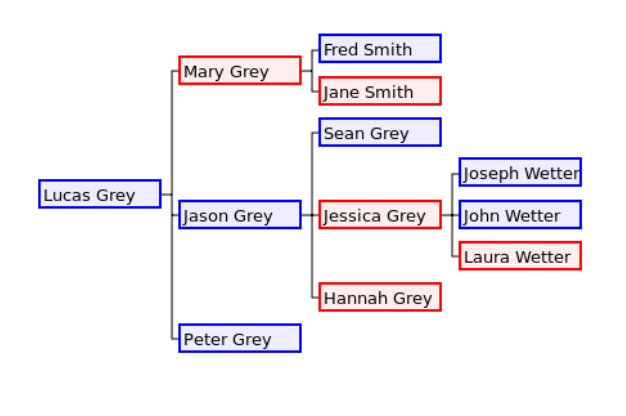
\includegraphics[scale=0.44]{treesEg2.png}
\end{center}
\end{frame}


\begin{frame}{Trees - Applications\footnote{\url{http://interactivepython.org/runestone/static/pythonds/Trees/trees.html}}}

\tblue{Taxonomy Tree:}
\begin{center}
    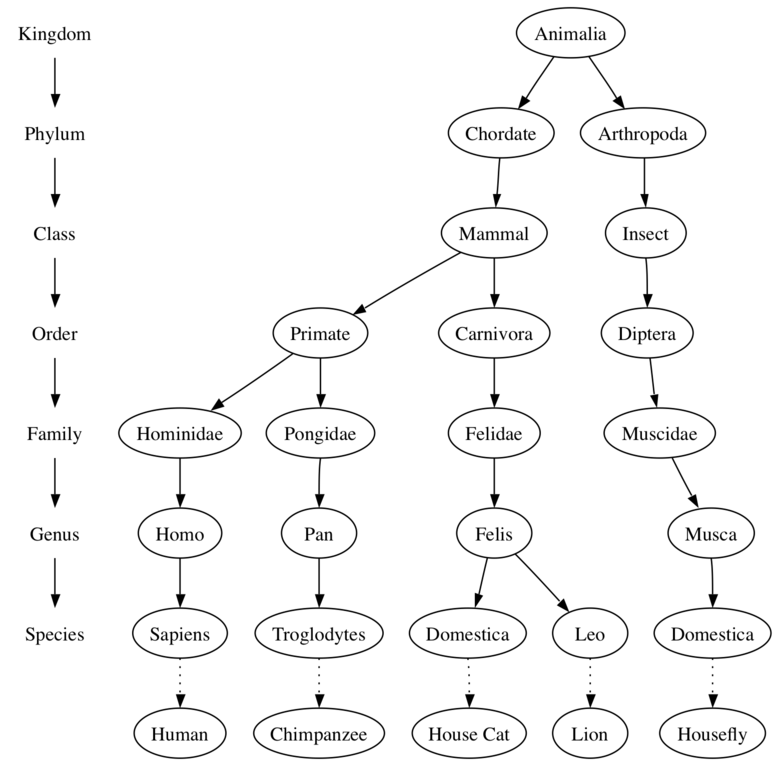
\includegraphics[scale=0.4]{treesEg1.png}
\end{center}
\end{frame}


\begin{frame}{Trees - Applications\footnote{\url{http://interactivepython.org/runestone/static/pythonds/Trees/trees.html}}}

\tblue{Directory Tree:}
\begin{center}
    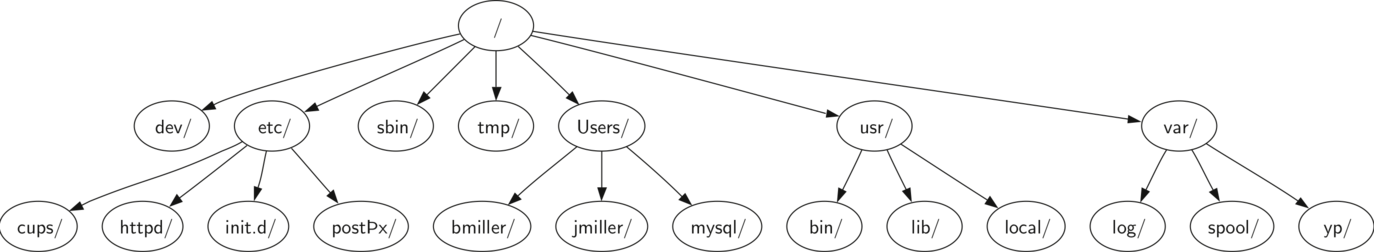
\includegraphics[scale=0.5]{treesEg3.png}
\end{center}
\end{frame}


\begin{frame}{Trees - Applications\footnote{\url{http://interactivepython.org/runestone/static/pythonds/Trees/trees.html}}}

\tblue{HTML DOM (Parse) Tree:}
\begin{center}
    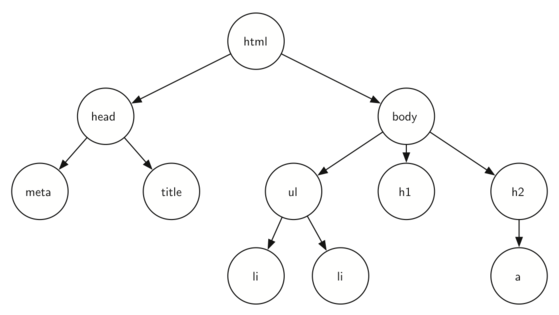
\includegraphics[scale=0.75]{treesEg4.png}
\end{center}
\end{frame}


\begin{frame}{Tree - Terminology}

\begin{columns}
    \column{0.5\textwidth}
            \begin{itemize}
            \item Node
            \item Edge
            \item Root
            \item Children 
            \item Parent 
            \item Sibling
            \item Subtree
            \item Leaf/External node
            \item Internal node
            \item Level (node) 
            \item Height (tree)
            \item Arity
            \end{itemize}
    \column{0.5\textwidth}
        \begin{center}
            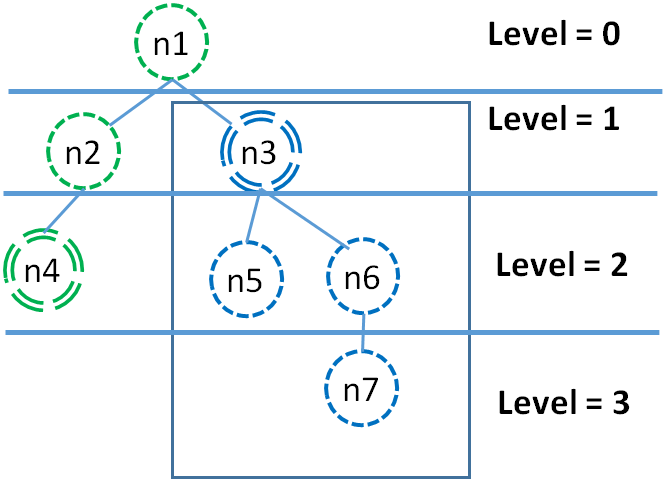
\includegraphics[scale=0.3]{treeTerminology.png}
        \end{center}
\end{columns}
\end{frame}


\begin{frame}{Tree - Abstract Representation\footnote{\url{http://interactivepython.org/runestone/static/pythonds/Trees/trees.html}}}
\begin{center}
    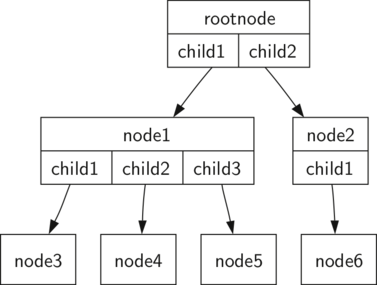
\includegraphics[scale=0.7]{treedef1.png}
\end{center}
\end{frame}


\section{BSTs}

\begin{frame}{Motivation}
    \begin{itemize}
        \item Store dynamic set efficiently
        \item Use good ideas from ordered list (OL) and ordered doubly linked list (ODLL)
        \item Use hierarchical storage to avoid pitfalls of OL and ODLL
        \item First attempt at hierarchical data structure that {\bf tries} to implement all 7 operations efficiently
    \end{itemize}
\end{frame}

\begin{frame}{Binary Trees}
    \begin{itemize}
        \item Each node has at most $2$ children
        \item Commonly referred to as {\em left} and {\em right} child
        \item The descendants of {\em left} child constitute {\em left} subtree
        \item The descendants of {\em right} child constitute {\em right} subtree
    \end{itemize}
\end{frame}

\begin{frame}{BST Property}
    \begin{itemize}
        \item For every node $x$, the keys of left subtree $\leq key(x)$
        \item For every node $x$, the keys of right subtree $\geq key(x)$
    \end{itemize}
    \begin{center}
        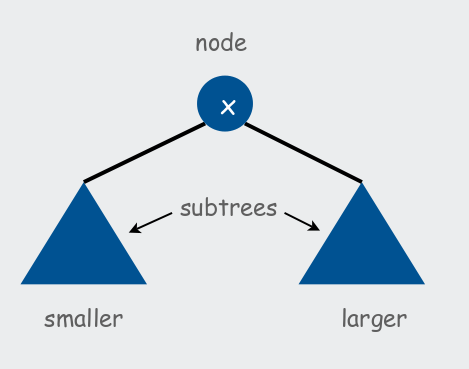
\includegraphics[scale=0.4]{bstProperty.png}\footnote{\url{http://www.cs.princeton.edu/~rs/AlgsDS07/08BinarySearchTrees.pdf}}
    \end{center}
\end{frame}


\begin{frame}{BST Examples\footnote{\url{http://en.wikipedia.org/wiki/Binary_search_tree}}}
    \begin{center}
        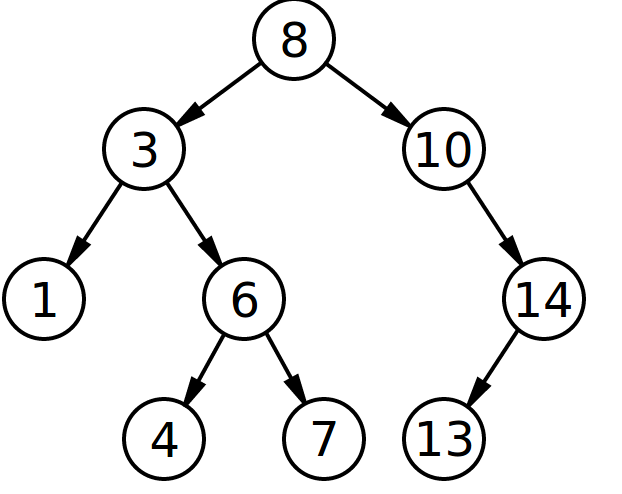
\includegraphics[scale=0.4]{bstExample.png}
    \end{center}
\end{frame}


\begin{frame}{BST Height\footnote{\url{https://engineering.purdue.edu/~ee608/handouts/lec10.pdf}}}
    \begin{itemize}
        \item There exists multiple possible BSTs to store same set of elements
        \item Minimum and Maximum Height: \pause $\lg n$ and $n$
        \item Best and worst case analysis (or specify analysis wrt height)
    \end{itemize}
    \begin{center}
        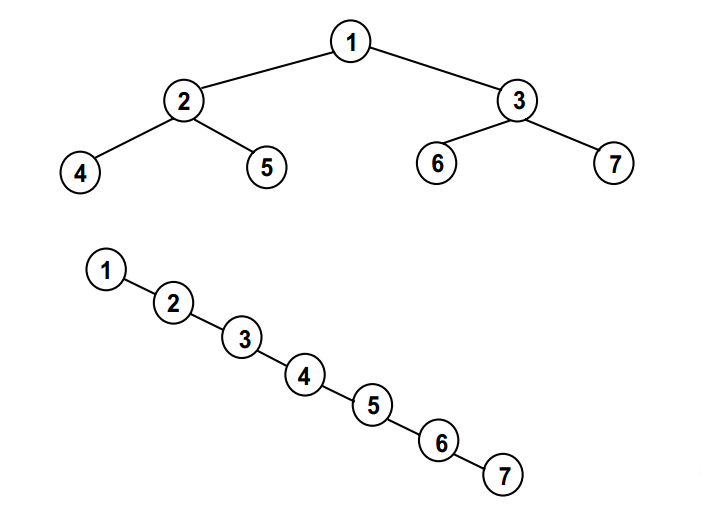
\includegraphics[scale=0.28]{bstMinMaxExamples.png}
    \end{center}
\end{frame}


\begin{frame}{Representation - I} 
    \begin{itemize}
        \item {\bf key:} Stores key information that is used to compare two nodes
        \item {\bf value:} Stores satellite/auxillary information
        \item {\bf parent:} Pointer to parent node. parent(root) = NULL
        \item {\bf left:} Pointer to left child if it exists. Else NULL
        \item {\bf right:} Pointer to right child if it exists. Else NULL
    \end{itemize}
\end{frame}


\begin{frame}{Representation - I\furl{CLRS Fig 10.9}}
    \begin{center}
        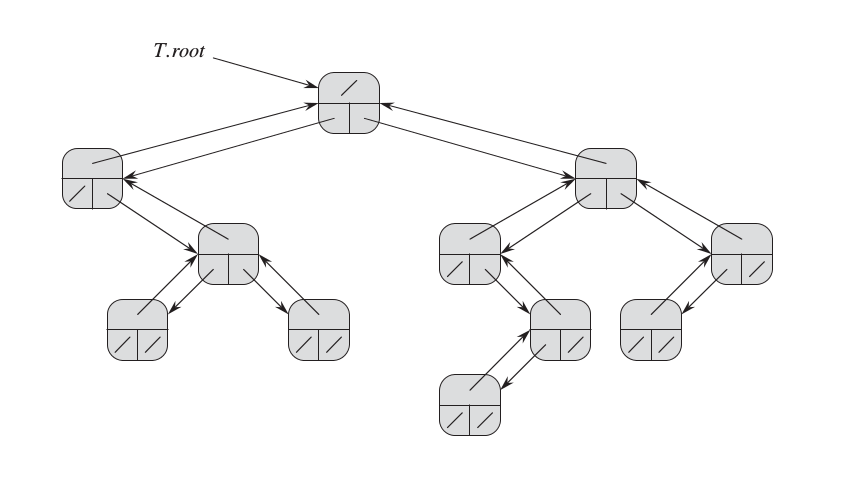
\includegraphics[scale=0.4]{bstRepresentation1.png}
    \end{center}
\end{frame}


\begin{frame}{Representation - II}
    \begin{center}
        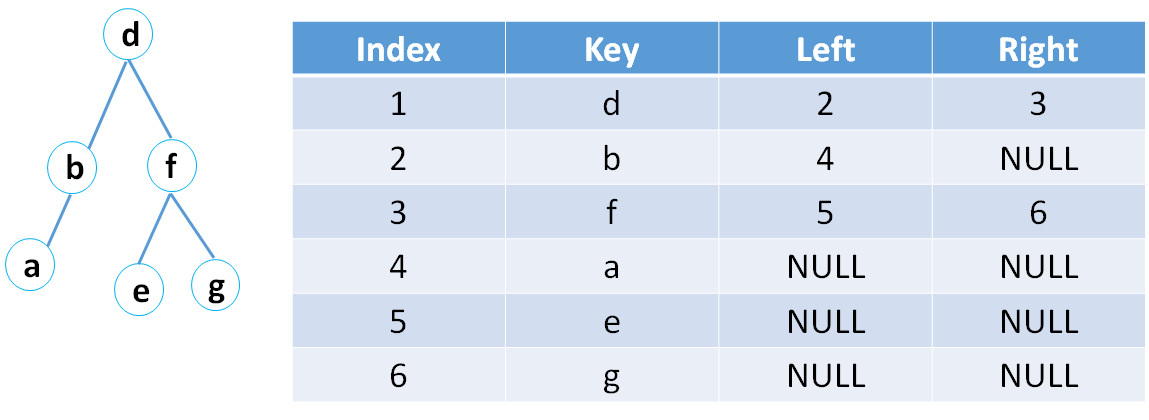
\includegraphics[scale=0.36]{bstRepresentation2.png}
    \end{center}
\end{frame}



\begin{frame}{Major Operations}
    \begin{itemize}
        \item Search
        \item Insert
        \item Minimum/Maximum
        \item Successor/Predecessor
        \item Deletion
        \item \hred{Traversals}
    \end{itemize}
\end{frame}

\begin{frame}{Key Helper Routines}
    \begin{itemize}
        \item Successor/Predecessor
        \item Traversals
        \item Case by Case Analysis:
        \begin{itemize}
            \item Analysis by number of children : $0, 1, 2$
            \item Analysis by type of children: {\em left}, {\em right}
        \end{itemize}
    \end{itemize}
\end{frame}

\begin{frame}{BST: Search}

\tblue{Search:} $4$
    \begin{center}
        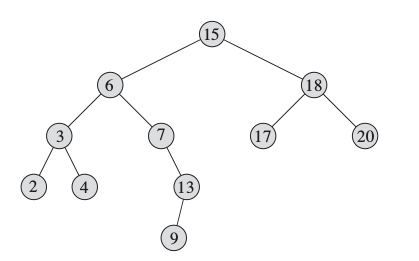
\includegraphics[scale=0.7]{bstSearch.png}
    \end{center}
\end{frame}


\begin{frame}{BST: Search}
    \begin{center}
        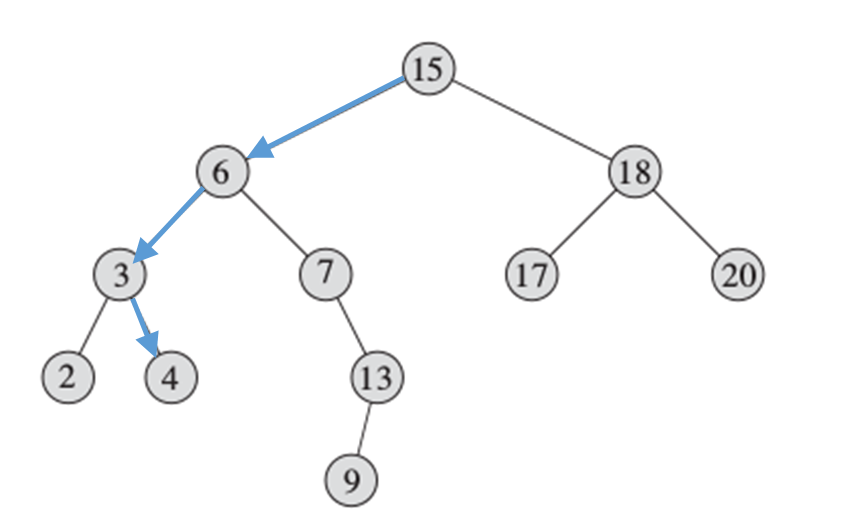
\includegraphics[scale=0.5]{bstSearch2.png}
    \end{center}
\end{frame}

\begin{frame}[fragile]{BST: Search}
    \begin{verbatim}
Tree-Search(x, k):
    if x == NULL or k == x.key
        return x
    if k < x.key
        return Tree-Search(x.left, k)
    else
        return Tree-Search(x.right, k)
    \end{verbatim}
    \begin{itemize}
        \item {\bf Analysis:} \pause $O(h)$
        \item {\bf Best Case:} $\lg n$ and {\bf Worst Case:} $O(n)$
    \end{itemize}
\end{frame}


\begin{frame}{BST: Insert}

\tblue{Insert:} $13$
    \begin{center}
        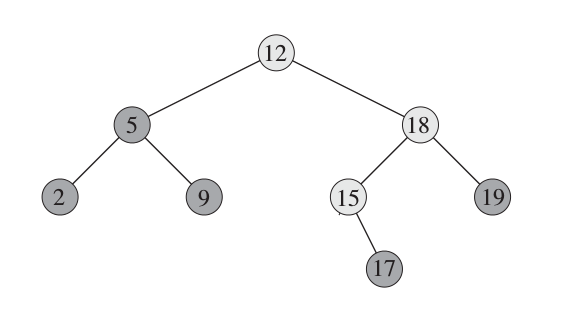
\includegraphics[scale=0.5]{bstInsert.png}
    \end{center}
\end{frame}


\begin{frame}{BST: Insert}

\tblue{Insert:} $13$
    \begin{center}
        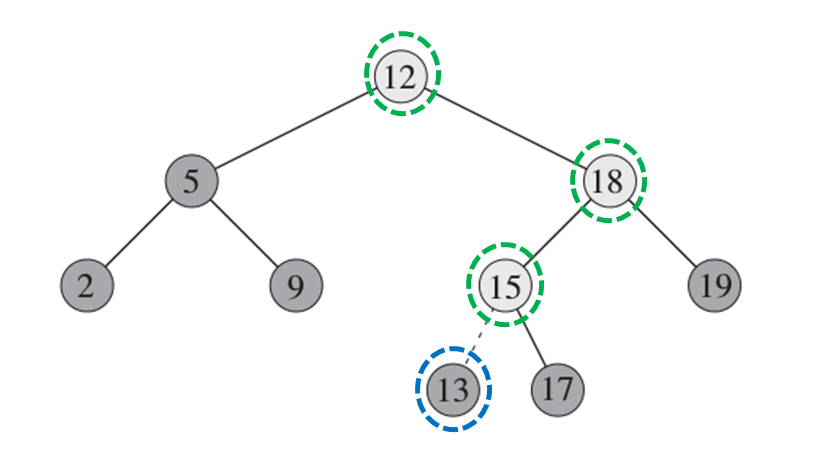
\includegraphics[scale=0.5]{bstInsert2.png}
    \end{center}
\end{frame}

\begin{frame}[fragile]{BST: }
    \begin{itemize}
        \item {\bf Analysis:} \pause $O(h)$ 
        \item {\bf Best Case:} $\lg n$ and {\bf Worst Case:} $O(n)$
    \end{itemize}
\end{frame}


\begin{frame}{BST: Minimum}

    \begin{center}
        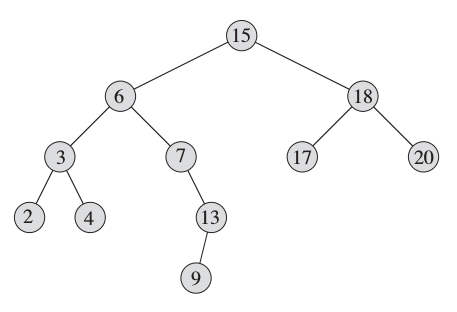
\includegraphics[scale=0.6]{bstMinimum.png}
    \end{center}
\end{frame}


\begin{frame}{BST: Minimum}

    \begin{center}
        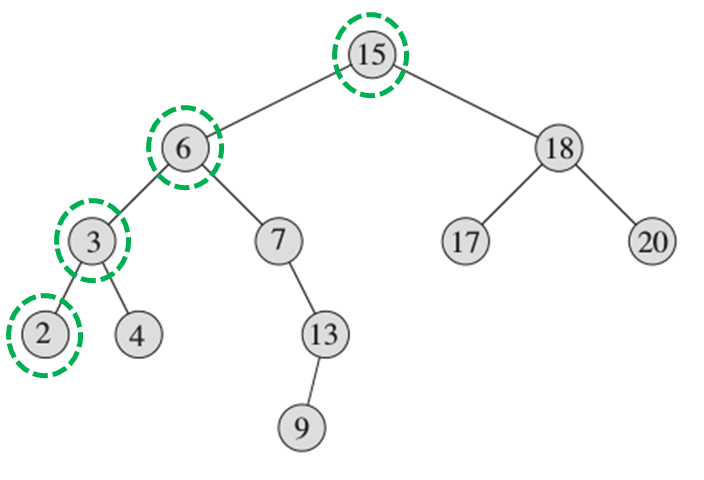
\includegraphics[scale=0.5]{bstMinimum2.png}
    \end{center}
\end{frame}

\begin{frame}[fragile]{BST: Minimum}
\begin{verbatim}
Tree-Minimum(x)
    while x.left is not NULL
        x = x.left
    return x
\end{verbatim}
    \begin{itemize}
        \item {\bf Analysis:} $O(h)$ 
        \item {\bf Best Case:} $\lg n$ and {\bf Worst Case:} $O(n)$
    \end{itemize}
\end{frame}


\begin{frame}{BST: Maximum}

    \begin{center}
        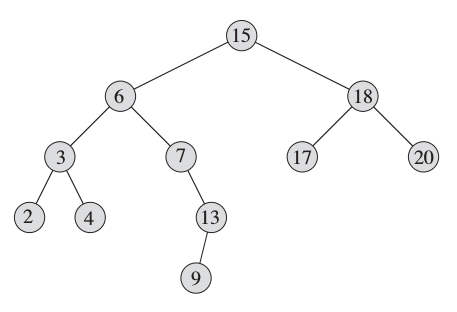
\includegraphics[scale=0.6]{bstMaximum.png}
    \end{center}
\end{frame}


\begin{frame}{BST: Maximum}

    \begin{center}
        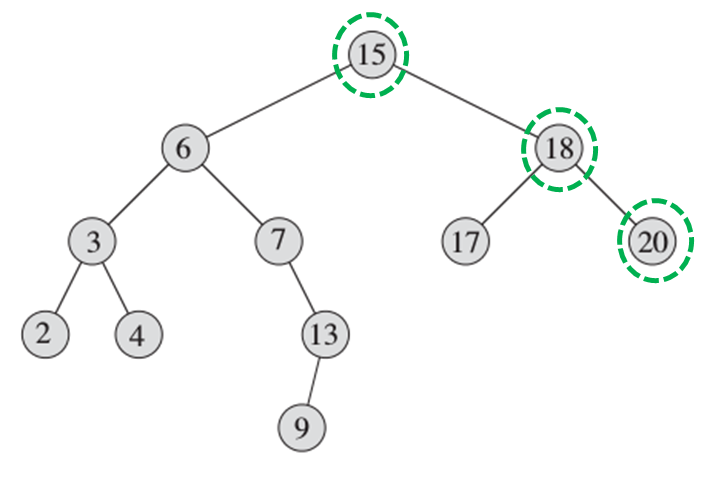
\includegraphics[scale=0.6]{bstMaximum2.png}
    \end{center}
\end{frame}

\begin{frame}[fragile]{BST: Maximum}
\begin{verbatim}
Tree-Maximum(x)
    while x.right is not NULL
        x = x.right
    return x
\end{verbatim}
    \begin{itemize}
        \item {\bf Analysis:} $O(h)$
        \item {\bf Best Case:} $\lg n$ and {\bf Worst Case:} $O(n)$
    \end{itemize}
\end{frame}


\begin{frame}{BST: Successor}

\tblue{Successor:} $15$
    \begin{center}
        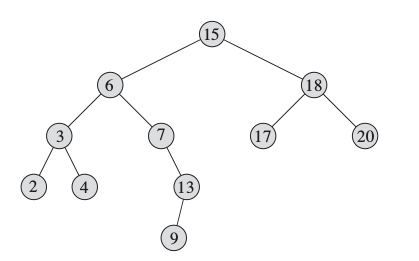
\includegraphics[scale=0.7]{bstSearch.png}
    \end{center}
\end{frame}


\begin{frame}{BST: Successor}

\tblue{Successor:} $15$
    \begin{center}
        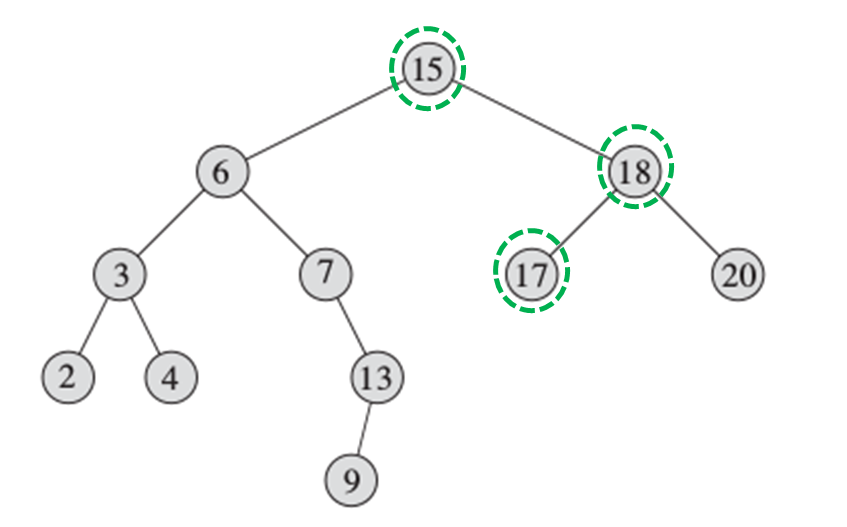
\includegraphics[scale=0.5]{bstSuccessor2.png}
    \end{center}
\end{frame}

\begin{frame}{BST: Successor}

\tblue{Successor:} $13$
    \begin{center}
        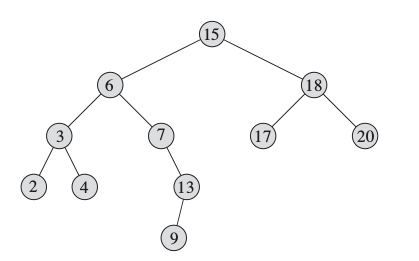
\includegraphics[scale=0.7]{bstSearch.png}
    \end{center}
\end{frame}


\begin{frame}{BST: Successor}

\tblue{Successor:} $13$
    \begin{center}
        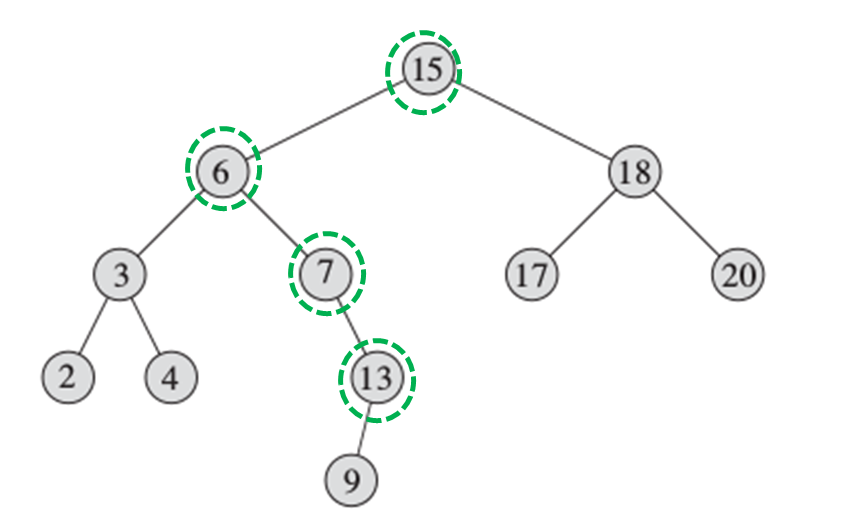
\includegraphics[scale=0.5]{bstSuccessor4.png}
    \end{center}
\end{frame}


\begin{frame}{BST: Successor}

    \begin{center}
        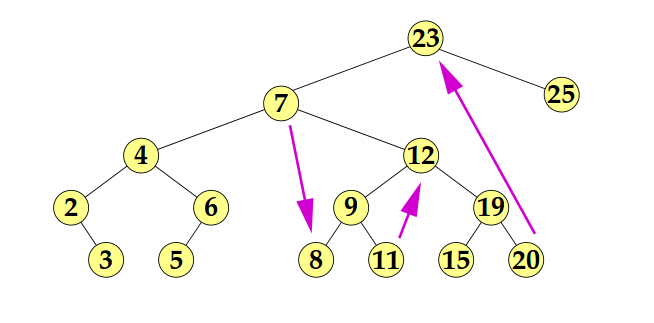
\includegraphics[scale=0.5]{bstSuccessor8.png}
    \end{center}
\end{frame}


\begin{frame}[fragile]{BST: }
\begin{verbatim}
Tree-Successor(x):
    if x.right is not NULL
        return Tree-Minimum(x.right)
    y = x.parent
    while y is not NULL and x == y.right
        x = y
        y = y.parent
    return y
\end{verbatim}
    \begin{itemize}
        \item BST Property allowed us to find successor {\bf without} comparing keys
        \item {\bf Analysis:} $O(h)$ 
        \item {\bf Best Case:} $\lg n$ and {\bf Worst Case:} $O(n)$
    \end{itemize}
\end{frame}



\begin{frame}{BST: Predecessor}

\tblue{Predecessor:} $6$
    \begin{center}
        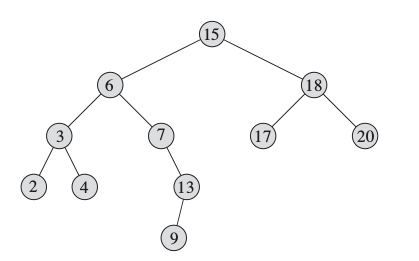
\includegraphics[scale=0.5]{bstSearch.png}
    \end{center}
\end{frame}


\begin{frame}{BST: Predecessor}

\tblue{Predecessor:} $6$
    \begin{center}
        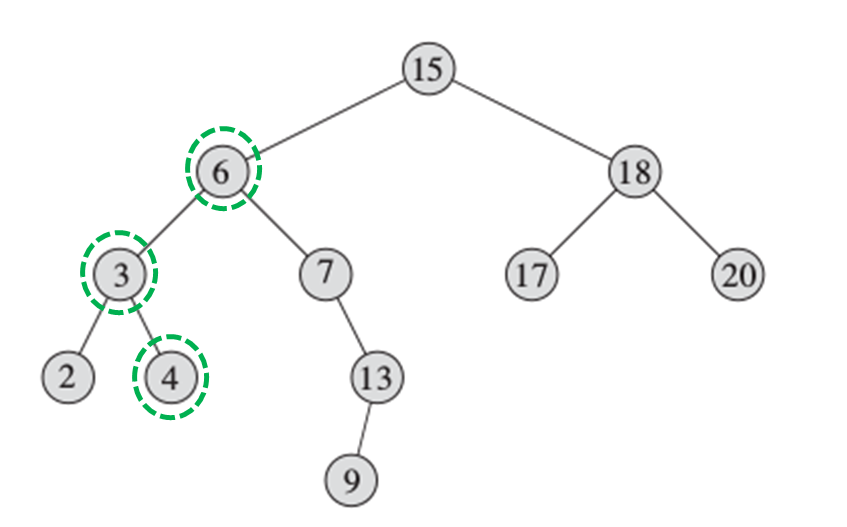
\includegraphics[scale=0.5]{bstPredecessor2.png}
    \end{center}
\end{frame}

\begin{frame}{BST: Predecessor}

\tblue{Predecessor:} $17$
    \begin{center}
        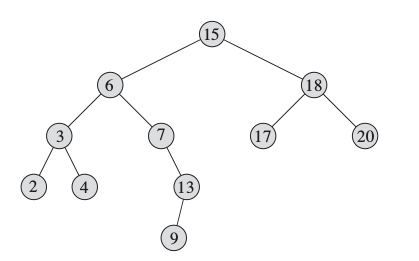
\includegraphics[scale=0.7]{bstSearch.png}
    \end{center}
\end{frame}


\begin{frame}{BST: Predecessor}

\tblue{Predecessor:} $17$
    \begin{center}
        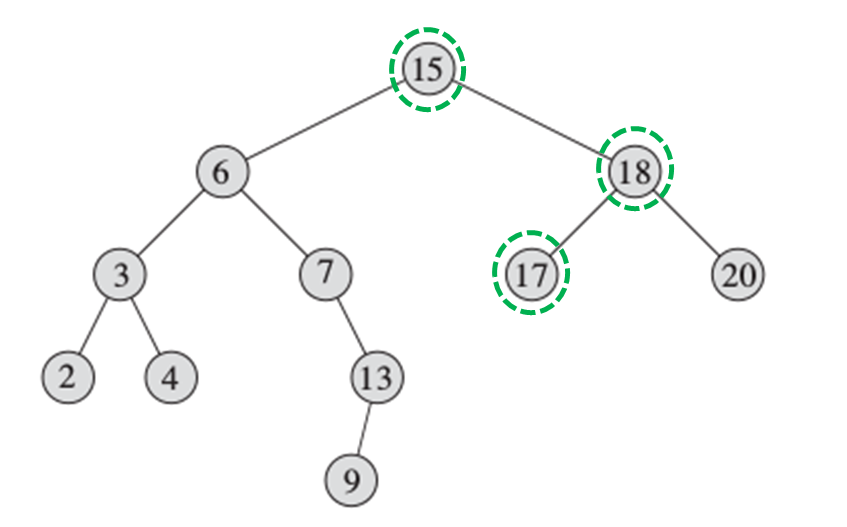
\includegraphics[scale=0.5]{bstPredecessor4.png}
    \end{center}
\end{frame}


\begin{frame}[fragile]{BST: }
\begin{verbatim}
Tree-Predecessor(x):
    if x.left is not NULL
        return Tree-Maximum(x.left)
    y = x.parent
    while y is not NULL and x == y.left
        x = y
        y = y.parent
    return y
\end{verbatim}
    \begin{itemize}
        \item BST Property allowed us to find predecessor {\bf without} comparing keys
        \item {\bf Analysis:} $O(h)$ 
        \item {\bf Best Case:} $\lg n$ and {\bf Worst Case:} $O(n)$
    \end{itemize}
\end{frame}

\begin{frame}{BST: Deletion}

    Trickiest Operation! Suppose we want to delete node $z$
    \begin{enumerate}
        \item $z$ has no children: Replace $z$ with NULL
        \item $z$ has one children $c$: Promote $c$ to $z$'s place
        \item $z$ has two children: 
        \begin{enumerate}
            \item[(a)] Let $z$'s successor be $y$
            \item[(b)] $y$ is either a leaf or has {\bf only} right child
            \item[(c)] Promote $y$ to $z$'s place
            \item[(d)] Fix $y$'s loss via Cases 1 or 2
        \end{enumerate}
    \end{enumerate}
\end{frame}


\begin{frame}{BST: Deletion Case I\furl{https://www.cs.rochester.edu/u/gildea/csc282/slides/C12-bst.pdf}}
    \begin{center}
        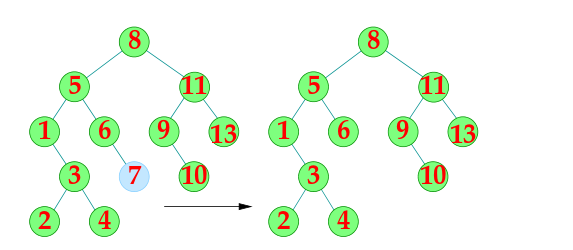
\includegraphics[scale=0.6]{bstDelCase1.png}
    \end{center}
\end{frame}


\begin{frame}{BST: Deletion Case II\furl{https://www.cs.rochester.edu/u/gildea/csc282/slides/C12-bst.pdf}}
    \begin{center}
        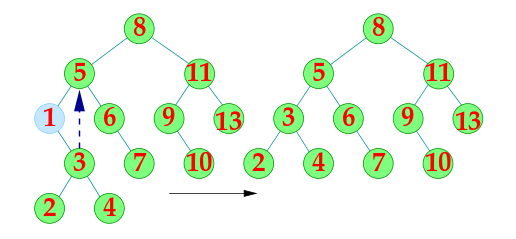
\includegraphics[scale=0.6]{bstDelCase2.png}
    \end{center}
\end{frame}


\begin{frame}{BST: Deletion Case III\furl{https://www.cs.rochester.edu/u/gildea/csc282/slides/C12-bst.pdf}}
    \begin{center}
        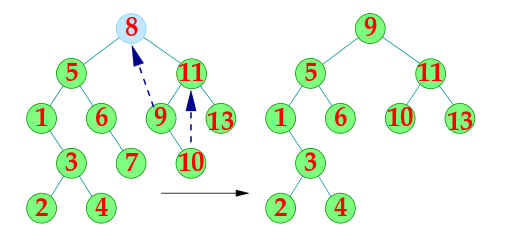
\includegraphics[scale=0.6]{bstDelCase3.png}
    \end{center}
\end{frame}


\begin{frame}{Digression}
    \begin{itemize}
        \item Perfectly fine if you cannot do deletion by memory
        \item Things will become hairier in RBT
        \item As long as you remember the key ideas and operations, you will be fine
    \end{itemize}
\end{frame}


\begin{frame}{BST: Traversal}
    \begin{itemize}
        \item {\bf Traversal:} Visit all nodes in a tree
        \item Many possible traversal strategies
        \item Three are most popular:  Pre-Order, In-Order, Post-Order
    \end{itemize}
    \begin{center}
        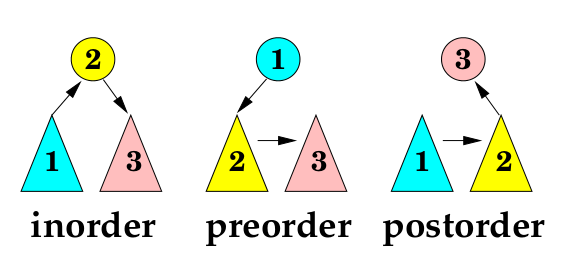
\includegraphics[scale=0.5]{bstTraversals.png}
    \end{center}
\end{frame}


\begin{frame}[fragile]{BST: Traversals}
\begin{verbatim}
In-Order-Walk(x):
    if x == NULL
        return
    In-Order-Walk(x.left)
    Print x.key
    In-Order-Walk(x.right)
\end{verbatim}
    \begin{itemize}
        \item {\bf Analysis:} \pause $O(n)$
        \item Holds true for all three traversals
    \end{itemize}
\end{frame}


\begin{frame}{BST: Traversal}
    \begin{center}
        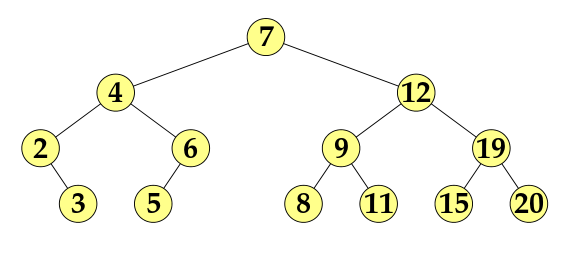
\includegraphics[scale=0.4]{bstTraversalEg.png}
    \end{center}
    \begin{itemize}
        \item {\bf In-Order:} \pause $2, 3, 4, 5, 6, 7, 8 , 9, 11, 12, 15, 19, 20$.
        \item {\bf Pre-Order:} \pause $7, 4, 2, 3, 6, 5, 12, 9, 8, 11, 19, 15, 20$.
        \item {\bf Pre-Order:} \pause $3, 2, 5, 6, 4, 8, 11, 9, 15, 20, 19, 12, 7$.
    \end{itemize}
\end{frame}


\begin{frame}{BST: Traversals}
    \begin{itemize}
        \item Notice anything special about In-Order traversal? \pause
        \begin{itemize}
            \item Returns items in sorted order!
        \end{itemize}
        \item Successor/Predecessor can be expressed in terms on In-Order traversal
    \end{itemize}
\end{frame}


\begin{frame}{Application: Tree-Sort}

    \tblue{Tree-Sort:}
    \begin{itemize}
        \item Construct a BST out of elements
        \item Do In-Order traversal
    \end{itemize}

    \tblue{Analysis:}
    \begin{itemize}
        \item {\bf Time Complexity:} Time Complexity for Constructing Tree + Time Complexity for In-Order traversal
        \item {\bf Best Case:} \pause $n \times \lg n + n$ = $O(n \lg n)$
        \item {\bf Worst Case:} \pause $n \times n + n$ = $O(n^2)$
    \end{itemize}
\end{frame}


\section{Balanced Binary Trees}

\begin{frame}{Balanced Binary Trees}
    \begin{itemize}
        \item Time complexity of BST operations depends on height
        \item Can vary between $O(\lg n)$ to $O(n)$
        \item BST operations do not take any special care to keep tree balanced
        \item If we can do the balancing efficiently, then all operations become faster
        \item Self-balancing - Do not run balancing algorithms periodically
    \end{itemize}
\end{frame}


\begin{frame}{Notion of Balance}
    \begin{itemize}
        \item Maintaining perfectly balanced trees is very hard and expensive
        \item So we resort to BSTs that are {\bf approximately} balanced
        \item Need to define notion of balance
        \item Ideas? \pause
        \begin{itemize}
            \item Informally, ensure the longest path in tree is not ``too'' long
            \item Many ways of formally specifying it
            \item Eg: $|$height(left subtree) $-$ height(right subtree)$|$ $\leq 1$ 
        \end{itemize}
        \item When can balance be broken? \pause Insertion, Deletion
    \end{itemize}
\end{frame}


\begin{frame}{Balanced Search Trees}
    \begin{itemize}
        \item Red-Black trees
        \item AVL trees
        \item $2-3$ and $2-3-4$ trees
        \item B-trees and other variants
        \item Treaps
        \item Skip trees
        \item Splay trees
        \item and many many more
    \end{itemize}
\end{frame}

\section{Red-Black Trees}
\begin{frame}{Red-Black Trees}
    \begin{center}
        \thblue{Red-Black Trees}
    \end{center}
\end{frame}


\begin{frame}{RBT: Motivation}
    \begin{itemize}
        \item Most important self-balancing BST
        \item Invented by Guibas-Sedgewick
        \item Simplifies/Unifies various balanced tree algorithms
        \item Became popular due to its simplicity in implementation
        \item Stores additional information about color of node ($1$ bit)
        \item All operations are logarithmic!
    \end{itemize}
\end{frame}


\begin{frame}{RBT Property}
    \begin{itemize}
        \item Every node is either red or black
        \item Root and leaves are black
        \item If node is red, then its parent is black
        \item All {\em simple} paths from any node $v$ to a descendent leaf have same number of black nodes. Aka {\em black-height($v$)}
    \end{itemize}
\end{frame}


\begin{frame}{RBT Example\footnote{MIT OCW 6-046j}}
    \begin{center}
        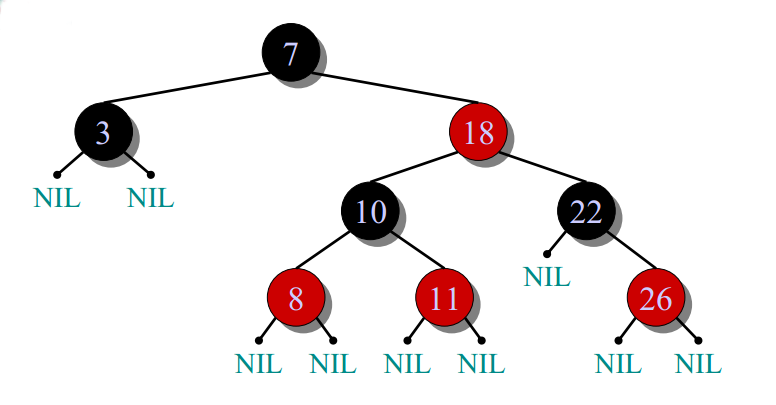
\includegraphics[scale=0.4]{rbtEg1.png}
    \end{center}
\end{frame}



\begin{frame}{RBT Example\footnote{MIT OCW 6-046j}}
    \begin{center}
        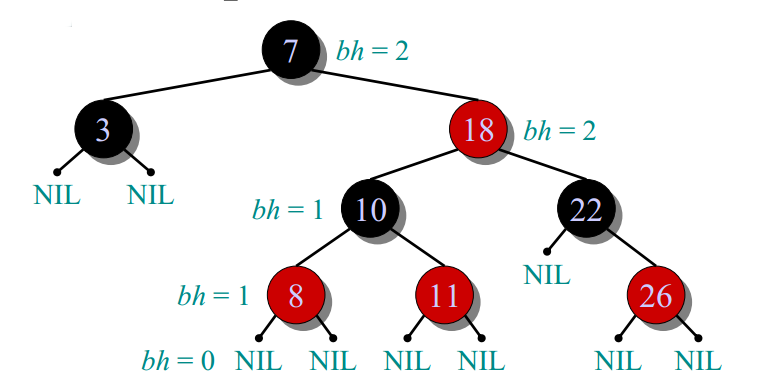
\includegraphics[scale=0.4]{rbtEg2.png}
    \end{center}
\end{frame}

\begin{frame}{RBT Property: Implications}
    \begin{itemize}
        \item If a {\bf red} node has any children, then it must have {\bf two} children and both must be {\bf black}
        \item If a {\bf black} node has {\bf only one} child, it has to be {\bf red}
        \item No root to leaf path has two consecutive red nodes
        \item No root to leaf path is more than twice as long as any other
        \item The rules {\bf bound} the imbalance in the tree
    \end{itemize}
\end{frame}


\begin{frame}{Major Operations}
    \begin{itemize}
        \item Search
        \item Insert
        \item Minimum/Maximum
        \item Successor/Predecessor
        \item Deletion
    \end{itemize}
\end{frame}

\begin{frame}{Key Helper Routines}
    \begin{itemize}
        \item Rotations - Right and Left
        \item Case by Case Analysis:
        \begin{itemize}
            \item Analysis by type of children, siblings and uncle (sibling of parent)
            \item Analysis by color of children
        \end{itemize}
    \end{itemize}
\end{frame}


\begin{frame}{RBT Theorem}
    \begin{theorem}[RBT Theorem]
        A red-black tree with $n$ keys has height 
            $$h \leq 2 \lg (n+1)$$
    \end{theorem}
    \begin{corollary}
        Operations Search, Min, Max, Successor, Predecessor all run in $O(\lg n)$ time  
        on a Red-Black tree with $n$ nodes.
    \end{corollary}
\end{frame}


\begin{frame}{RBT - Modifying Operations}
    \begin{itemize}
        \item Insert and Delete need to be more complex so as to balance the tree
        \item They cause ``changes'' to tree
        \begin{itemize}
            \item Change of color (recoloring)
            \item Change of tree structure via ``rotations''
        \end{itemize}
    \end{itemize}
\end{frame}


\begin{frame}{Rotations\footnote{MIT OCW 6-046j}}
    \begin{center}
        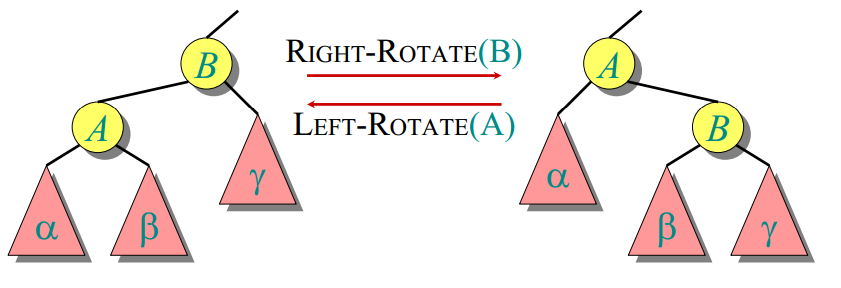
\includegraphics[scale=0.4]{rotationsEg.png}
    \end{center}
    \begin{itemize}
        \item Rotation can be done in $O(1)$ time. 
        \item Rotations maintain in-order ordering of keys: 
            $a \in \alpha, b \in \beta, c \in \gamma \Rightarrow a \leq A \leq b \leq B \leq c$
    \end{itemize}
\end{frame}


\begin{frame}{RBT Insertion }
    \begin{itemize}
        \item Insert $z$ in tree (based on BST property)
        \item Color $z$ red
        \item Only red-black property $3$ can be violated
        \item Fix violations by rotations and recoloring
    \end{itemize}
\end{frame}

\begin{frame}{RBT : Insertion\footnote{\url{http://web.cse.ohio-state.edu/~lai/2331/0.Red-Black\%20Trees.pdf}}}
    \begin{itemize}
        \item Case I: The parent and ``uncle'' of $z$ are both red
        \begin{itemize}
            \item Color parent and uncle of $z$ as black
            \item Color grandparent of $z$ as red
            \item Recurse of grandparent of $z$
        \end{itemize}
    \end{itemize}
    \begin{center}
        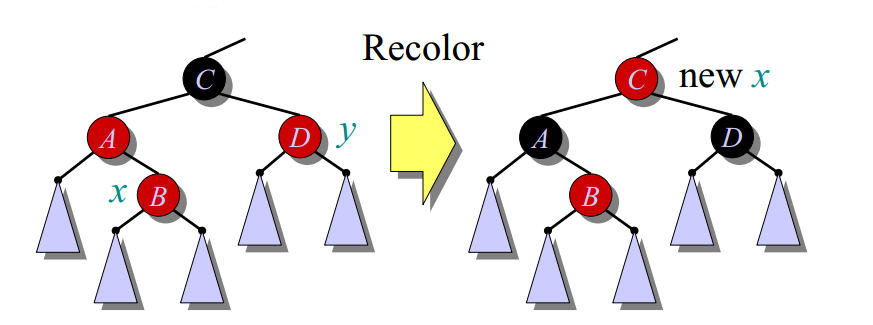
\includegraphics[scale=0.4]{rbtInsertEg1.png}
    \end{center}
\end{frame}


\begin{frame}{RBT : Insertion\footnote{\url{http://web.cse.ohio-state.edu/~lai/2331/0.Red-Black\%20Trees.pdf}}}
    \begin{itemize}
        \item Case II: The parent of $z$ is red, the uncle of $z$ is black, $z$'s parent is a left child , $z$ is a right child
        \begin{itemize}
            \item Left rotate on $z$'s parent
            \item Make $z$'s left child the new $z$
            \item Solve this scenario by using by Case III
        \end{itemize}
    \end{itemize}
    \begin{center}
        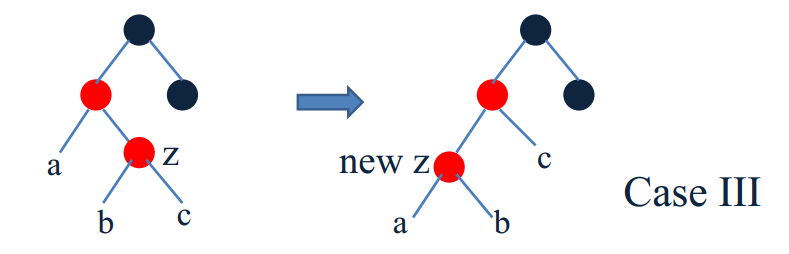
\includegraphics[scale=0.4]{rbtInsertEg2.png}
    \end{center}
\end{frame}


\begin{frame}{RBT : Insertion\footnote{\url{http://web.cse.ohio-state.edu/~lai/2331/0.Red-Black\%20Trees.pdf}}}
    \begin{itemize}
        \item Case III: The parent of $z$ is Red and the uncle is black, $z$ is a left child, and its parent is a left child
        \begin{itemize}
            \item Right rotate on grandparent of $z$
            \item Switch colors of $z$'s parent and $z$'s sibling
            \item Done!
        \end{itemize}
    \end{itemize}
    \begin{center}
        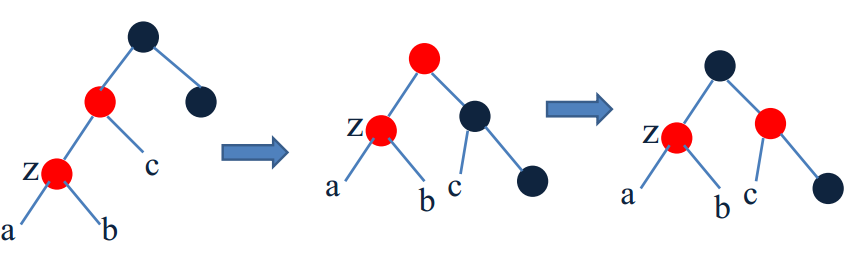
\includegraphics[scale=0.38]{rbtInsertEg3.png}
    \end{center}
\end{frame}


\begin{frame}{RBT : Insertion\footnote{\url{http://web.cse.ohio-state.edu/~lai/2331/0.Red-Black\%20Trees.pdf}}}
    \begin{itemize}
        \item Case II': Symmetric to Case II
    \end{itemize}
    \begin{center}
        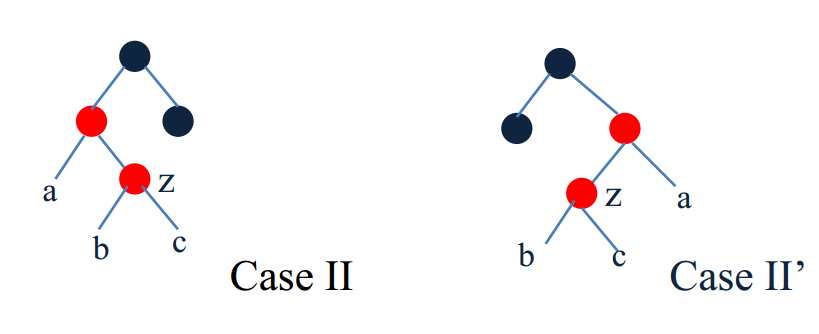
\includegraphics[scale=0.4]{rbtInsertEg4.png}
    \end{center}
\end{frame}


\begin{frame}{RBT : Insertion\footnote{\url{http://web.cse.ohio-state.edu/~lai/2331/0.Red-Black\%20Trees.pdf}}}
    \begin{itemize}
        \item Case III': Symmetric to Case III
    \end{itemize}
    \begin{center}
        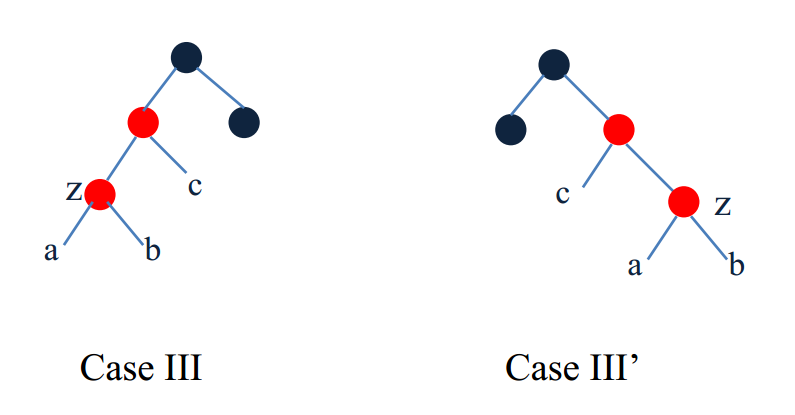
\includegraphics[scale=0.4]{rbtInsertEg5.png}
    \end{center}
\end{frame}

\begin{frame}{RBT : Insertion Sorted Elements}
    \begin{itemize}
        \item Refer \url{https://www.cs.utexas.edu/~scottm/cs314/handouts/slides/Topic23RedBlackTrees.pdf} for a step-by-step example of how RBT handles insertion in sorted order
    \end{itemize}
\end{frame}

\begin{frame}{RBT: Deletion}
    \begin{itemize}
        \item Similarly complicated 
        \item Refer to CLRS book for full details
    \end{itemize}
\end{frame}

\section{Summary}
\begin{frame}{Summary}

\tblue{Major Concepts:}
\begin{itemize}
\item Binary Search Trees
\item Concept of Self-Balancing
\item Red-Black Trees
\end{itemize}
\end{frame}


\end{document}

